\documentclass{beamer}
\usepackage{amsmath}
\usepackage{amssymb}
\usepackage{bbm}
\usepackage{pgf}
\usepackage{tikz}
\usepackage{nicefrac}
\usetikzlibrary{matrix}
\usetheme{boxes}
\newcommand{\fig}{figures} % common figure path
\newcommand{\frnzplt}{FranzPlot }
\newcommand{\dbbslsh}{\textbackslash \textbackslash} % common figure path
\newcommand{\norm}[1]{\left\lVert#1\right\rVert}
\newcommand{\parallelsum}{\mathbin{\!/\mkern-5mu/\!}}
\DeclareMathSymbol{\shortminus}{\mathbin}{AMSa}{"39}


\title[Curve e Sup. - Lab 3]{Curve e Superfici per il Design \\ Laboratorio - 2}
\author[Prof. Parolini]{Prof. Nicola Parolini}
%\institute[dimat]{Long Inst.}
\date{31 Ottobre 2019}

\begin{document}
\begin{frame}
\maketitle
\end{frame}

\begin{frame}
\frametitle{Materiali}
Il materiale per l'esercitazione di oggi:
\begin{itemize}
\item Questa presentazione \\ (\texttt{Materiale Didattico/Laboratori/lab 3/lab3\_testo.pdf});
%\item Il file \texttt{es\_dado\_ref.toml} con l'esercizio risolto della passata esercitazione.
\item L'eseguibile del \frnzplt \\ (\texttt{Software/Franzplot 19.08 - Windows.exe})
\end{itemize}
\end{frame}

\begin{frame}
\frametitle{Rotazioni: Asse x}
\begin{equation}
R_x(\theta) = 
\begin{bmatrix}
1 & 0 & 0 \\
0 & \mbox{cos}(\theta) & - \mbox{sen}(\theta)\\
0 & \mbox{sen}(\theta) & \mbox{cos}(\theta)
\end{bmatrix}
\end{equation}
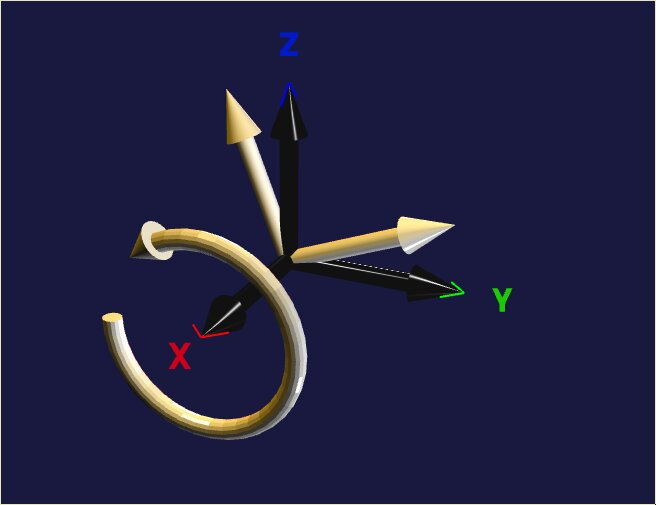
\includegraphics[width=0.6\textwidth]{\fig/rot_x.jpeg}
\end{frame}
\begin{frame}
\frametitle{Rotazioni: Asse y}
\begin{equation}
R_y(\theta) = 
\begin{bmatrix}
\mbox{cos}(\theta) & 0 & \mbox{sen}(\theta)\\
0 & 1 & 0 \\
-\mbox{sen}(\theta)& 0 & \mbox{cos}(\theta)
\end{bmatrix}
\end{equation}
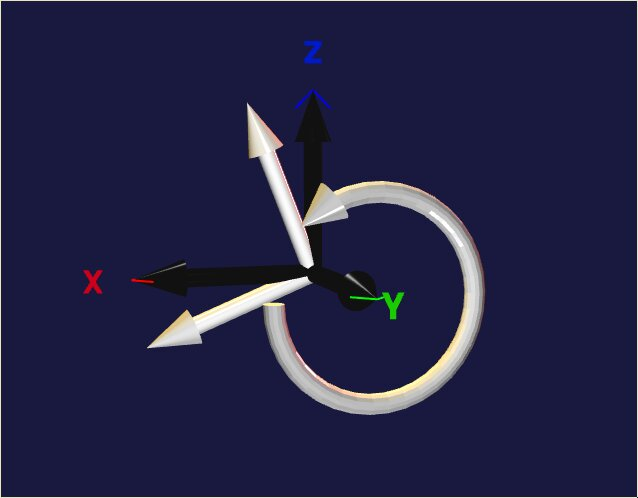
\includegraphics[width=0.6\textwidth]{\fig/rot_y.jpeg}
\end{frame}
\begin{frame}
\frametitle{Rotazioni: Asse z}
\begin{equation}
R_z(\theta) = 
\begin{bmatrix}
\mbox{cos}(\theta) & - \mbox{sen}(\theta) & 0\\
\mbox{sen}(\theta) & \mbox{cos}(\theta)   & 0\\ 
0 & 0 & 1 
\end{bmatrix}
\end{equation}
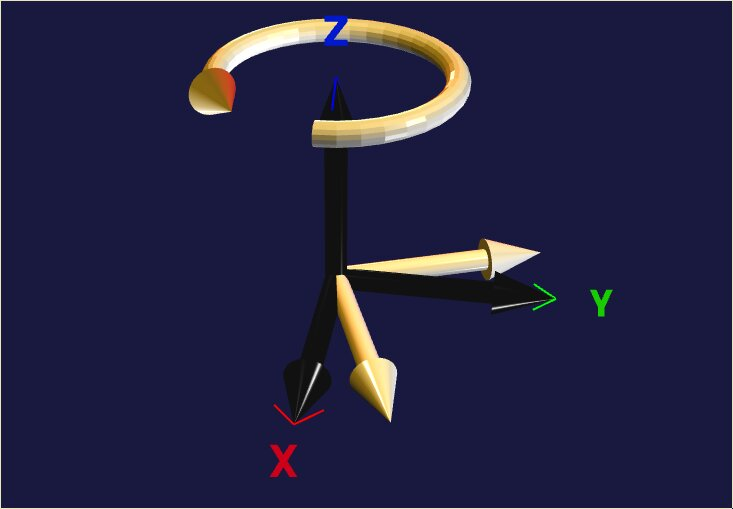
\includegraphics[width=0.6\textwidth]{\fig/rot_z.jpeg}
\end{frame}
%
\begin{frame}
\frametitle{Tagli}
\begin{columns}
\begin{column}{0.48\textwidth}
Taglio in direzione x sulle facce con normale y:
\begin{equation}
T_{xy}=\begin{bmatrix}
    1 & k_x & 0\\
    0 & 1   & 0\\
    0 & 0   & 1
    \end{bmatrix}
\end{equation}
\end{column}
\begin{column}{0.48\textwidth}
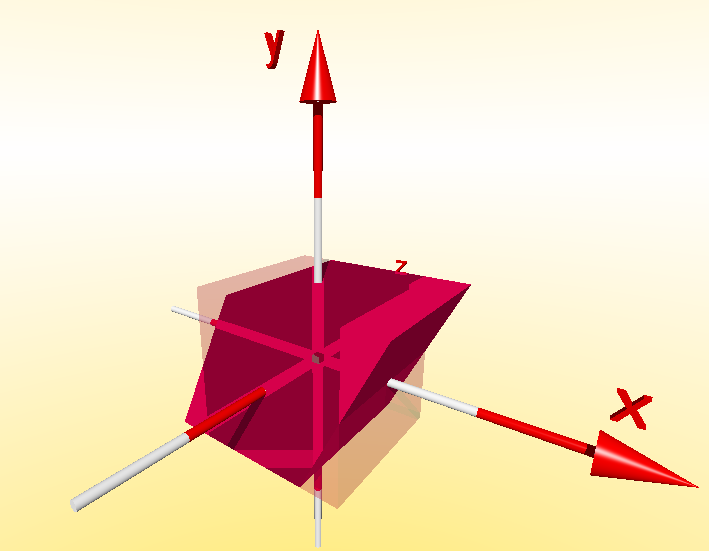
\includegraphics[width=0.8\textwidth]{\fig/cut_tx.png}
\end{column}
\end{columns}
%
\begin{columns}
\begin{column}{0.48\textwidth}
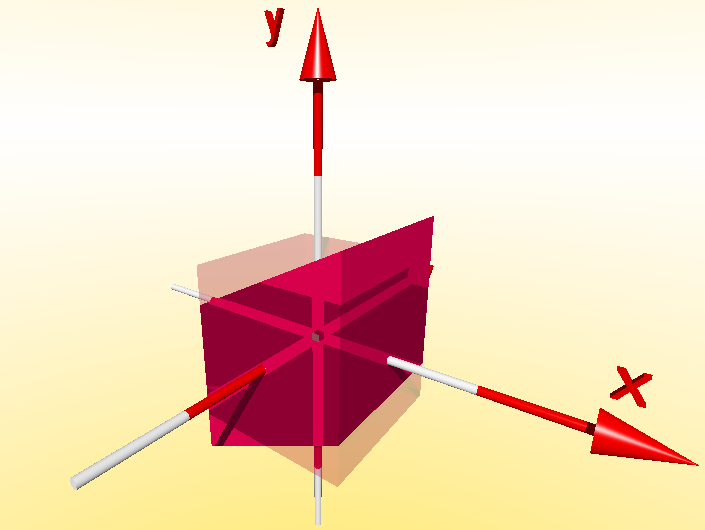
\includegraphics[width=0.8\textwidth]{\fig/cut_ty.png}
\end{column}
\begin{column}{0.48\textwidth}
Taglio in direzione y sulle facce con normale x:
\begin{equation}
T_{yx}=\begin{bmatrix}
    1   & 0 & 0\\
    k_y & 1 & 0\\
    0   & 0 & 1
    \end{bmatrix}
\end{equation}
\end{column}
\end{columns}
\end{frame}
%
\begin{frame}
\frametitle{Tagli[2]}
\begin{columns}
\begin{column}{0.48\textwidth}
Taglio in direzione z sulle facce con normale x:
\begin{equation}
T_{zx}=\begin{bmatrix}
    1 & 0 & 0\\
    0 & 1 & 0\\
    k_z & 0 & 1
    \end{bmatrix}
\end{equation}
\end{column}
\begin{column}{0.48\textwidth}
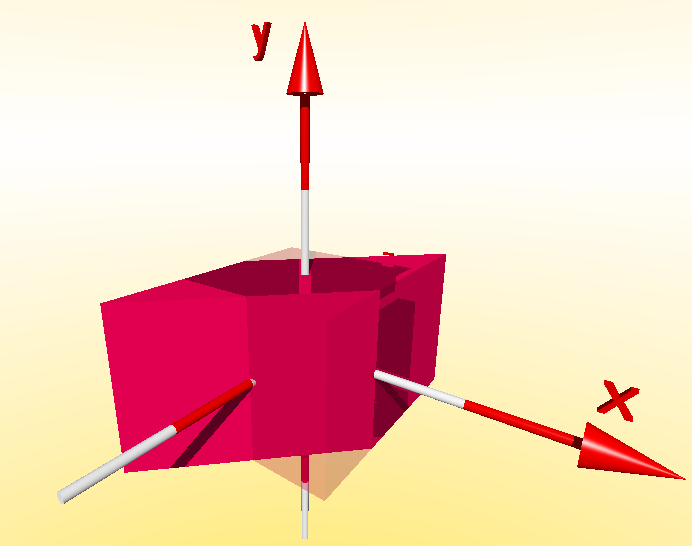
\includegraphics[width=0.8\textwidth]{\fig/cut_tz-x.png}
\end{column}
\end{columns}
%
%\begin{block}{}
\begin{columns}
\begin{column}{0.48\textwidth}
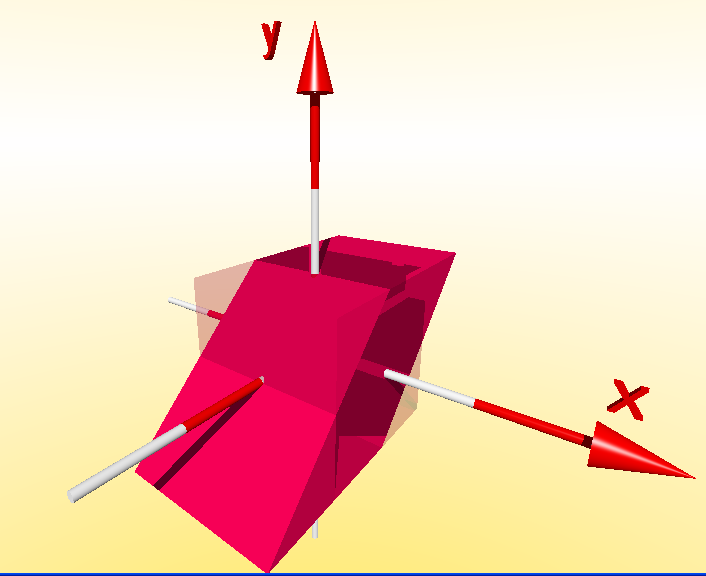
\includegraphics[width=0.8\textwidth]{\fig/cut_tz-y.png}
\end{column}
\begin{column}{0.48\textwidth}
Taglio in direzione z sulle facce con normale y:
\begin{equation}
T_{zy}=\begin{bmatrix}
    1 & 0 & 0\\
    0 & 1 & 0\\
    0 & k_z & 1
    \end{bmatrix}
\end{equation}
\end{column}
\end{columns}
%\end{block}
\end{frame}
%
\begin{frame}
\frametitle{Scalatura, Riflessione,Proiezione}
\begin{itemize}
\item Scalatura
\begin{equation}
S = \begin{bmatrix}
    S_x & 0 & 0\\
    0 & S_y & 0\\
    0 & 0 & S_z
    \end{bmatrix}
\end{equation}
\item Riflessione
\begin{equation}
F = \begin{bmatrix}
      1 & 0 & 0\\
      0 & 1 & 0\\
      0 & 0 & 1
    \end{bmatrix}
    -2~\begin{bmatrix}
    n_x \\
    n_y \\
    n_z
    \end{bmatrix} 
    ~\begin{bmatrix}
    n_x & n_y & n_z
    \end{bmatrix}
\end{equation}
\item Proiezione
\begin{equation}
 P = \begin{bmatrix}
      1 & 0 & 0\\
      0 & 1 & 0\\
      0 & 0 & 1
    \end{bmatrix}
    -\begin{bmatrix}
    n_x \\
    n_y \\
    n_z
    \end{bmatrix} 
    ~\begin{bmatrix}
    n_x & n_y & n_z
    \end{bmatrix}
\end{equation}
\end{itemize}
\end{frame}
%
\begin{frame}
\frametitle{Coordinate omogenee}
\begin{displaymath}
\begin{bmatrix}
a_{11} & a_{12} & a_{13} & t_1 \\
a_{21} & a_{22} & a_{23} & t_2 \\
a_{31} & a_{32} & a_{33} & t_3 \\
0      &    0   &  0     & 1 
\end{bmatrix}
~\begin{bmatrix}
x \\ y\\ z\\ 1
\end{bmatrix}
=  
\begin{bmatrix}
a_{11}x + a_{12}y + a_{13}z + t_1 \\
a_{21}x + a_{22}y + a_{23}z + t_2 \\
a_{31}x + a_{32}y + a_{33}z + t_3 \\
 1
\end{bmatrix}
\end{displaymath}
\end{frame}



\section{Esercizi}
%
\begin{frame}
\frametitle{Esercizio 1 - Moltiplicazioni matrice-matrice}
Date le due matrici:
\begin{displaymath}
    A =
\begin{bmatrix}
   1 &  2 &  0 &  0 \\
  -2 &  1 &  0 &  1 \\
   3 &  0 &  1 & -1 \\
   0 &  0 &  0 &  1
\end{bmatrix}
\qquad
B = 
\begin{bmatrix}
   1 &  0 &  3 &  1 \\
   2 &  1 &  0 &  1 \\
   2 &  0 & -3 &  0 \\
   0 &  0 &  0 &  1 
\end{bmatrix}
\end{displaymath}
\begin{itemize}
\item Calcolare la matrice $M = A B$
\item Calcolare la matrice $N = B A$
\end{itemize}
\end{frame}
%
\begin{frame}
\frametitle{Esercizio 1 - i}
Calcolo di M:
\begin{displaymath}
    M =
\begin{bmatrix}
   1 &  2 &  0 &  0 \\
  -2 &  1 &  0 &  1 \\
   3 &  0 &  1 & -1 \\
   0 &  0 &  0 &  1
\end{bmatrix}
\begin{bmatrix}
   1 &  0 &  3 &  1 \\
   2 &  1 &  0 &  1 \\
   2 &  0 & -3 &  0 \\
   0 &  0 &  0 &  1 
\end{bmatrix}
\end{displaymath}

La matrice M risultante sar\`a una matrice $4\times4$, e dobbiamo calcolarla elemento per elemento:

\begin{displaymath}
    M =
\begin{bmatrix}
    M_{11} & M_{12} & M_{13} & M_{14} \\
    M_{21} & M_{22} & M_{23} & M_{24} \\
    M_{31} & M_{32} & M_{33} & M_{34} \\
    M_{41} & M_{42} & M_{43} & M_{44}
\end{bmatrix}
\end{displaymath}

\end{frame}

\begin{frame}
\frametitle{Esercizio 1 - ii}

    L'elemento $M_{ij}$, ovvero quel numero contenuto nella matrice M e posizionato nella \textbf{riga i} e nella
    \textbf{colonna j}, \`e il \textbf{prodotto scalare} dei vettori \textbf{riga i-esima di A} e \textbf{colonna j-esima di B}


Vediamo il calcolo di alcuni elementi di matrice:
\begin{displaymath}
    M_{11} =
\begin{bmatrix}
    1 &  2 &  0 &  0
\end{bmatrix}
\cdot
\begin{bmatrix}
    1 \\  2 \\ 2 \\ 0
\end{bmatrix}
 = 1 \cdot 1 + 2 \cdot 2 + 0 \cdot 2 + 0 \cdot 0
 = 5
\end{displaymath}

\end{frame}

\begin{frame}
\frametitle{Esercizio 1 - iii}

\begin{displaymath}
    M_{21} =
\begin{bmatrix}
    -2 & 1 &  0 &  1
\end{bmatrix}
\cdot
\begin{bmatrix}
    1 \\  2 \\ 2 \\ 0
\end{bmatrix}
 = \shortminus 2 \cdot 1 + 1 \cdot 2 + 0 \cdot 2 + 1 \cdot 0
 = 0
\end{displaymath}


\begin{displaymath}
    M_{23} =
\begin{bmatrix}
    -2 & 1 &  0 &  1
\end{bmatrix}
\cdot
\begin{bmatrix}
    3 \\  0 \\ -3 \\ 0
\end{bmatrix}
 = \shortminus 2 \cdot 3 + 1 \cdot 0 + 0 \cdot \shortminus 3 + 1 \cdot 0
 = \shortminus 6
\end{displaymath}

E cos\`i via per tutti gli altri elementi.
\end{frame}

\begin{frame}
\frametitle{Esercizio 1 - iv}

Poich\'e ogni singolo elemento di matrice richiede il calcolo di un prodotto scalare di due vettori,
    per calcolare la matrice $M$ dovremo calcolare $\mathbf{16}$ prodotti scalari.
    \begin{itemize}
        \item Allenarsi nel calcolo a mente dei prodotti scalari ci permette di non 
            consumare quantit\`a industriali di carta.
    \end{itemize}
    Nei nostri esercizi in genere le matrici contengono molti zeri, questo semplifica molto i calcoli.
    \begin{itemize}
        \item In particolare, quando lavoriamo in coordinate omogenee \textbf{l'ultima riga} di una
            qualsiasi matrice di trasformazione \`e sempre 
$\begin{bmatrix} 0 & 0 &  0 &  1 \end{bmatrix}  $
    \end{itemize}

\end{frame}
%
\begin{frame}
\frametitle{Esercizio 1}
\begin{itemize}
    \item Creare un oggetto `dado' e traslarlo del vettore $[1, 1, 0]^T$.
    \item Scrivere la matrice T che descrive la rotazione di 180 gradi intorno all'asse Z.
    \item Applicare la matrice T calcolata in precedenza al dado traslato, usando il nodo
        ``Generic Matrix''.
    \item Scrivere una matrice di rotazione in cui l'angolo sia una variabile tempo-dipendente $t$. Inserire questa matrice in un nodo "Time Transform"
        per verificare che il senso di rotazione sia quello corretto (rispetti la regola della mano destra).
\end{itemize}
\end{frame}

\begin{frame}
\frametitle{Esercizio 1 - i}
Matrice generica di rotazione intorno l'asse Z:
\begin{equation*}
R_z(\theta) = 
\begin{bmatrix}
\mbox{cos}(\theta) & - \mbox{sin}(\theta) & 0\\
\mbox{sin}(\theta) & \mbox{cos}(\theta)   & 0\\ 
0 & 0 & 1 
\end{bmatrix}
\end{equation*}
    Nel nostro caso, $\theta = \pi$. Andiamo quindi a sostituire per ottenere
\begin{equation*}
T = 
\begin{bmatrix}
\mbox{cos}(\pi) & - \mbox{sin}(\pi) & 0\\
\mbox{sin}(\pi) & \mbox{cos}(\pi)   & 0\\ 
0 & 0 & 1 
\end{bmatrix}
\end{equation*}
    Sappiamo anche che $cos(\pi) = -1$ e $sin(\pi) = 0$.\\ 
    La matrice che cerchiamo \`e quindi:
\begin{equation*}
T = 
\begin{bmatrix}
-1 & 0 & 0\\
0 & -1  & 0\\ 
0 & 0 & 1 
\end{bmatrix}
\end{equation*}
\end{frame}

%\begin{frame}
%Il grafo che descrive la scena:
%    \vspace{0.5cm}
%\begin{center}
%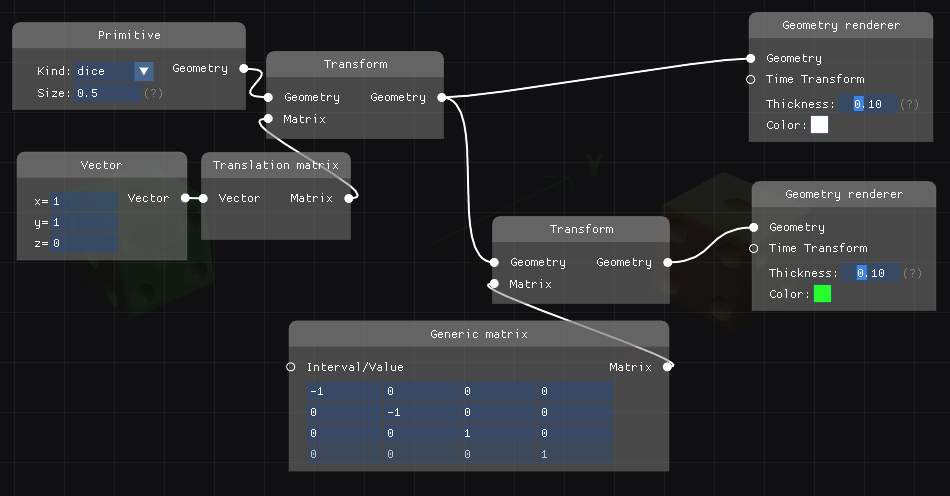
\includegraphics[width=\textwidth]{\fig/lab2_es1_a.png}
%\end{center}
%\end{frame}

\begin{frame}
\frametitle{Esercizio 1 - ii}
\begin{center}
\begin{tikzpicture}
\node(img1){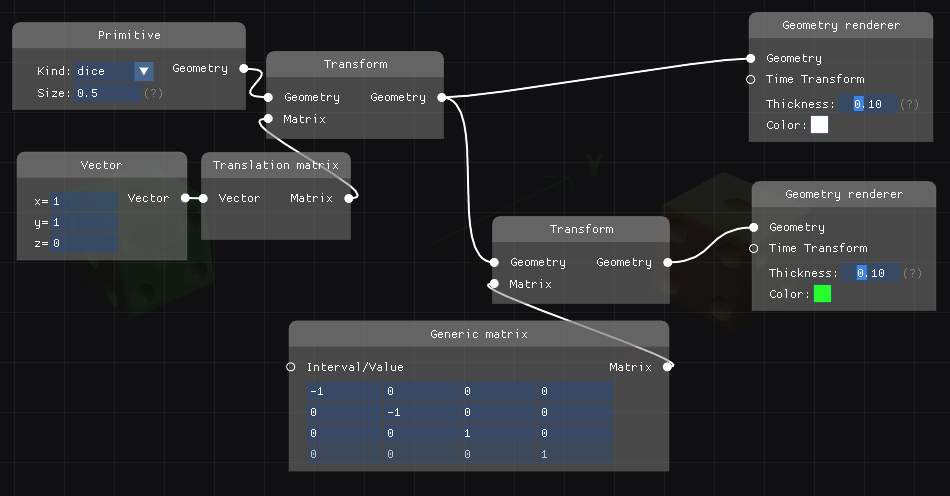
\includegraphics[width=0.85\textwidth]{\fig/lab2_es1_a.png}};
\node(img2) at (img1.south east){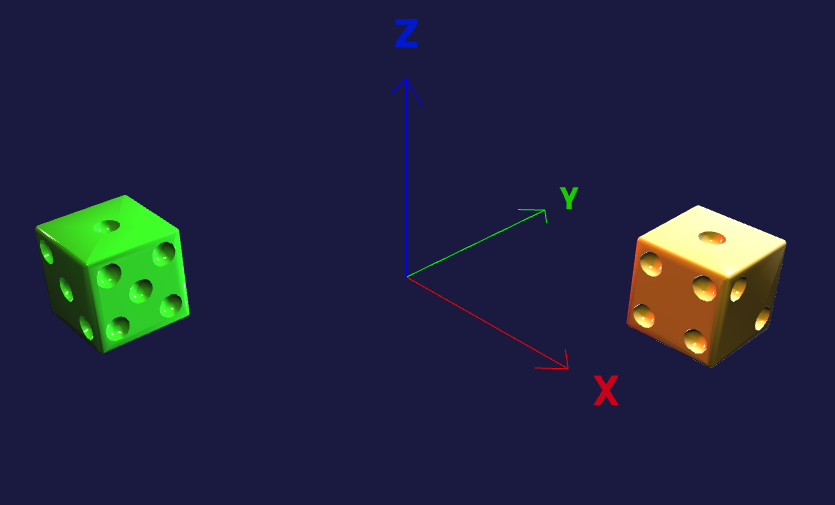
\includegraphics[width=0.45\textwidth]{\fig/lab2_es1_b.png}};
\end{tikzpicture}
\end{center}
\end{frame}

\begin{frame}
\frametitle{Esercizio 1 - iii}
Riscriviamo la matrice, ma come angolo scriviamo la variabile $t$:
\begin{equation*}
\begin{bmatrix}
\mbox{cos}(t) & - \mbox{sin}(t) & 0\\
\mbox{sin}(t) & \mbox{cos}(t)   & 0\\ 
0 & 0 & 1 
\end{bmatrix}
\end{equation*}
e la inseriamo nel nodo ``Time Transform''

    \vspace{0.2cm}
\centering
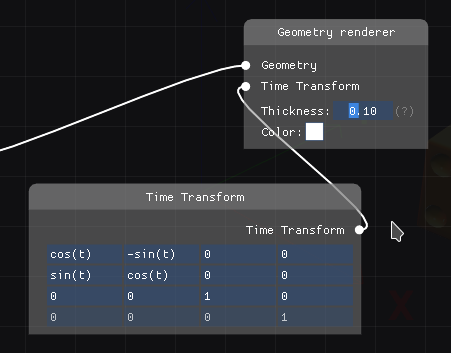
\includegraphics[width=0.5\textwidth]{\fig/lab2_es1_c.png}
\end{frame}

\begin{frame}
\frametitle {Esercizio 2}
\begin{itemize}
    \item Creare un oggetto `dado' e traslarlo del vettore $v = [1, 1, 0]^T$.
    \item Scrivere la matrice R che descrive la riflessione rispetto al piano passante per l'origine e avente vettore normale $v$
    \item Applicare la matrice R al dado traslato, usando il nodo
        ``Generic Matrix''.
    \item Rappresentare il dado traslato, il dado riflesso e il piano di riflessione.
    \item Scrivere la matrice $Q = \mathbb{I} - 2t\hat{v}\hat{v}^T$, con $t$ variabile tempo-dipendente. Inserire questa matrice in un nodo
        ``Time Transform'' e animare la scena con $t$ che va da $0$ a $1$. Commentare il risultato.
    \item Confrontare l'oggetto finale ottenuto in questo esercizio con quello ottenuto nell'esercizio precedente.
\end{itemize}
\end{frame}
\begin{frame}
\frametitle{ Esercizio 2 - i}
    Matrice di riflessione generica (quando $\mathbf{n}$ \`e il \textbf{versore} normale)
\begin{equation}
F = \begin{bmatrix}
      1 & 0 & 0\\
      0 & 1 & 0\\
      0 & 0 & 1
    \end{bmatrix}
    -2~\begin{bmatrix}
    n_x \\
    n_y \\
    n_z
    \end{bmatrix} 
    ~\begin{bmatrix}
    n_x & n_y & n_z
    \end{bmatrix}
\end{equation}
    Nel nostro caso, $\mathbf{v}$ \`e il vettore normale, \textbf{non il versore!} \\
    $\Rightarrow$ dobbiamo prima ricavare $\hat{v}$ versore!
\end{frame}

\begin{frame}
\frametitle{ Esercizio 2 - ii}
Ricordando la definizione:
    \begin{equation*}
    \hat{v} = \frac{\mathbf{v}}{\norm{\mathbf{v}}}
    \end{equation*}
calcoliamo
    \begin{equation*}
    \norm{\mathbf{v}} = \sqrt{1^2 + 1^2 + 0^2} = \sqrt{2}
    \end{equation*}
e otteniamo
\begin{displaymath}
\hat{v} =
    \frac{1}{\sqrt{2}}
    \begin{bmatrix}
    1 \\
    1 \\
    0
                \end{bmatrix}
=  \begin{bmatrix}
    \nicefrac{1}{\sqrt{2}}\\
    \nicefrac{1}{\sqrt{2}}\\
                0
                \end{bmatrix}
\end{displaymath}
\end{frame}

\begin{frame}
\frametitle{ Esercizio 2 - iii}
La matrice di riflessione cercata diventa dunque:
\begin{displaymath}
\mathcal{R} =  \begin{bmatrix}
                1 & 0 & 0\\
                0  & 1 & 0\\
                0 & 0 & 1
                \end{bmatrix}
    -2~\begin{bmatrix}
    \nicefrac{1}{\sqrt{2}} \\
    \nicefrac{1}{\sqrt{2}} \\
    0
    \end{bmatrix} 
    ~\begin{bmatrix}
    \nicefrac{1}{\sqrt{2}} & \nicefrac{1}{\sqrt{2}} & 0
    \end{bmatrix}
\end{displaymath}

\begin{displaymath}
\mathcal{R} =  \begin{bmatrix}
                1 & 0 & 0\\
                0  & 1 & 0\\
                0 & 0 & 1
                \end{bmatrix}
    -2~\begin{bmatrix}
                \nicefrac{1}{2} & \nicefrac{1}{2}  & 0\\
                \nicefrac{1}{2} & \nicefrac{1}{2}  & 0\\
                0 & 0 & 0
                \end{bmatrix}
\end{displaymath}

\begin{displaymath}
\mathcal{R} =  \begin{bmatrix}
                1 & 0 & 0\\
                0  & 1 & 0\\
                0 & 0 & 1
                \end{bmatrix}
    -\begin{bmatrix}
                1 & 1 & 0\\
                1 & 1 & 0\\
                0 & 0 & 0
                \end{bmatrix}
 =  \begin{bmatrix}
                0 & -1 & 0\\
                -1 & 0 & 0\\
                0 & 0 & 1
                \end{bmatrix}
\end{displaymath}
\end{frame}

\begin{frame}
\frametitle{Esercizio 2 - iv}
\begin{center}
\begin{tikzpicture}
\node(img1){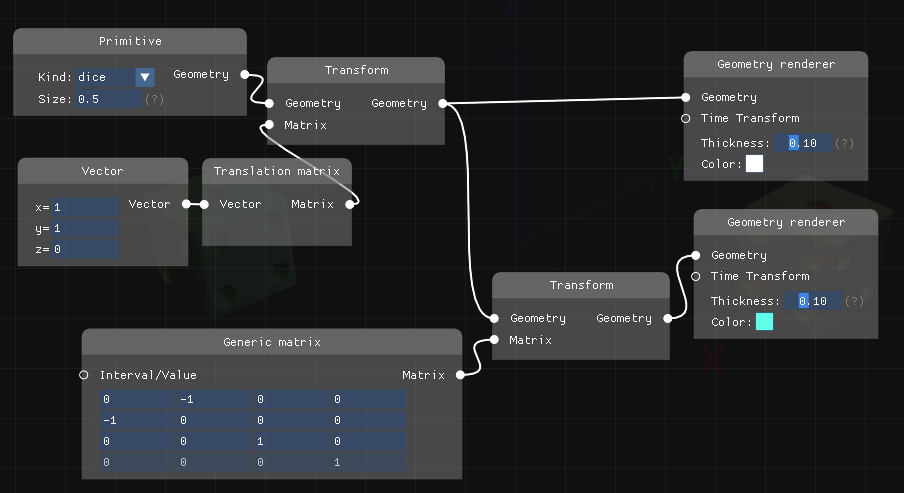
\includegraphics[width=0.85\textwidth]{\fig/lab2_es2_a.png}};
\node(img2) at (img1.south east){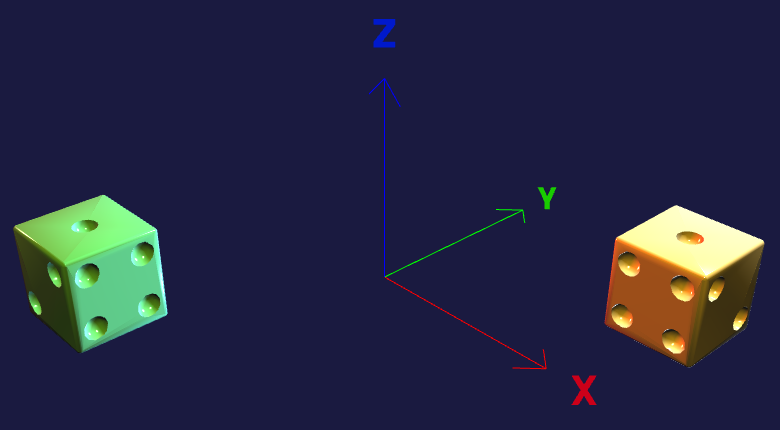
\includegraphics[width=0.45\textwidth]{\fig/lab2_es2_b.png}};
\end{tikzpicture}
\end{center}
\end{frame}

\begin{frame}
\frametitle{ Esercizio 2 - v}
    Il calcolo di $Q = \mathbb{I} - 2t\hat{v}\hat{v}^T$ \`e molto simile, dobbiamo solo stare attenti a $t$:
\begin{displaymath}
Q =  \begin{bmatrix}
                1 & 0 & 0\\
                0  & 1 & 0\\
                0 & 0 & 1
                \end{bmatrix}
    -2t\begin{bmatrix}
    \nicefrac{1}{\sqrt{2}} \\
    \nicefrac{1}{\sqrt{2}} \\
    0
    \end{bmatrix} 
    ~\begin{bmatrix}
    \nicefrac{1}{\sqrt{2}} & \nicefrac{1}{\sqrt{2}} & 0
    \end{bmatrix}
\end{displaymath}

\begin{displaymath}
Q =  \begin{bmatrix}
                1 & 0 & 0\\
                0  & 1 & 0\\
                0 & 0 & 1
                \end{bmatrix}
    -2t\begin{bmatrix}
                \nicefrac{1}{2} & \nicefrac{1}{2}  & 0\\
                \nicefrac{1}{2} & \nicefrac{1}{2}  & 0\\
                0 & 0 & 0
                \end{bmatrix}
\end{displaymath}

\begin{displaymath}
Q =  \begin{bmatrix}
                1 & 0 & 0\\
                0  & 1 & 0\\
                0 & 0 & 1
                \end{bmatrix}
    -\begin{bmatrix}
                t & t & 0\\
                t & t & 0\\
                0 & 0 & 0
                \end{bmatrix}
 =  \begin{bmatrix}
                1 - t & -t & 0\\
                -t & 1 - t & 0\\
                0 & 0 & 1
                \end{bmatrix}
\end{displaymath}
\end{frame}

\begin{frame}
\frametitle{Esercizio 2 - vi}
    Confrontiamo questo risultato (sx) con quello precedente (dx)
    \begin{center}
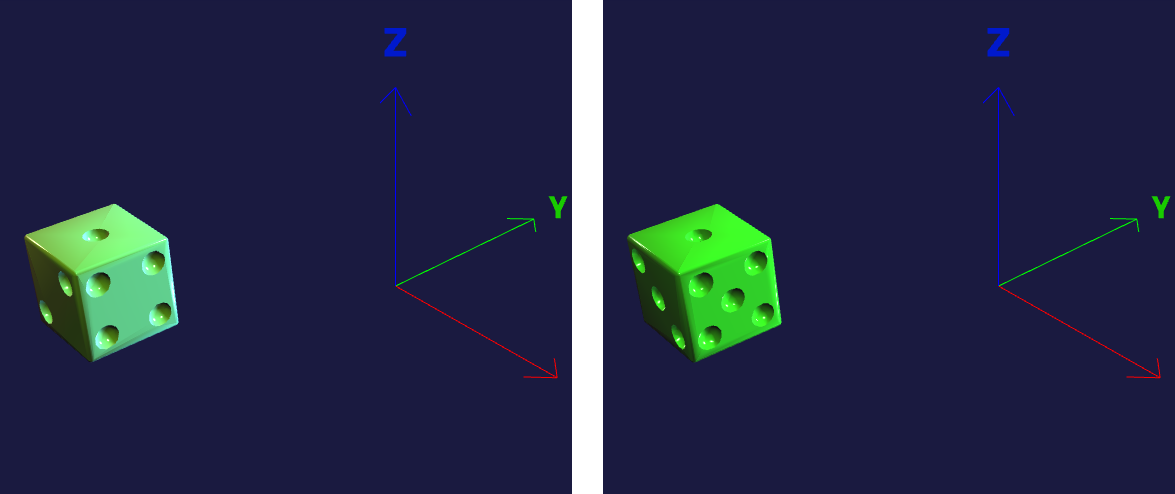
\includegraphics[width=0.9\textwidth]{\fig/lab2_es2_comparison.png}
    \end{center}
    Il dado si trova nella stessa posizione, ma le facce sono orientate
    in maniera diversa. La riflessione ne ha cambiato l'ordine! \\
    Ruotando la scena ottenuta in questo esercizio si pu\`o verificare che l'ordine nel dado originale \`e
    2-3-5-4, nel dado riflesso \`e 2-4-5-3.
\end{frame}

\begin{frame}
\frametitle{Esercizio 3}
        Dati i due vettori $\mathbf{u} = [0, 1, 2]^T$ e $\mathbf{v} = [0, -3, 1]^T$:
\begin{itemize}
    \item Determinare se i due vettori siano paralleli.
    \item Determinare se i due vettori siano perpendicolari tra loro.
    \item Rappresentare nel \frnzplt i due vettori, spiccandoli entrambi dall'origine degli assi.
\end{itemize}
\end{frame}

\begin{frame}

\frametitle{Esercizio 3 - i}
 $\mathbf{u} \parallelsum \mathbf{v} \quad \Leftrightarrow \quad \exists t \in \mathbb R, t\neq 0,\ \text{tale che } \mathbf u = t\mathbf v$

\begin{equation*}
 \left\{
 \begin{array}{l}
  u_x = t\cdot v_x \\
  u_y = t\cdot v_y \\
  u_z = t\cdot v_z
 \end{array}
 \right. 
 \quad \rightarrow \quad
  \left\{
 \begin{array}{l}
  0 = 0\ t \\
  1 = -3\ t \\
  2 = 1\ t
 \end{array}
 \right.
 \quad \rightarrow \quad
  \left\{
 \begin{array}{l}
  \mathit{nessuna\ informazione} \\
  t = \nicefrac{-1}{3} \\
  t = 2
 \end{array}
 \right.
\end{equation*}
La seconda e terza equazione sono in contraddizione, pertanto non esiste alcuna $t$ che soddisfi il sistema lineare \\
$\Rightarrow$ $\mathbf{u}$ e $\mathbf{v}$ non sono paralleli.
\end{frame}

\begin{frame}

\frametitle{Esercizio 3 - ii}
$\mathbf{u} \perp \mathbf{v} \quad \Leftrightarrow \quad \mathbf u \cdot \mathbf v = 0$

\begin{displaymath}
\mathbf u \cdot \mathbf v =  \begin{bmatrix}
                0 \\
                1 \\
                2 
                \end{bmatrix}
    \cdot \begin{bmatrix}
                0 \\
                -3\\
                1
                \end{bmatrix}
\end{displaymath}

\begin{displaymath}
\mathbf u \cdot \mathbf v
 =  0 \cdot 0 + 1 \cdot (-3) + 2 \cdot 1 = -1
\end{displaymath}
Poich\'e il prodotto scalare dei due vettori \`e diverso da zero, sappiamo
che essi non sono perpendicolari.
\end{frame}

\begin{frame}
\frametitle{Esercizio 3 - iii}
\vspace{-0.5cm}
\begin{center}
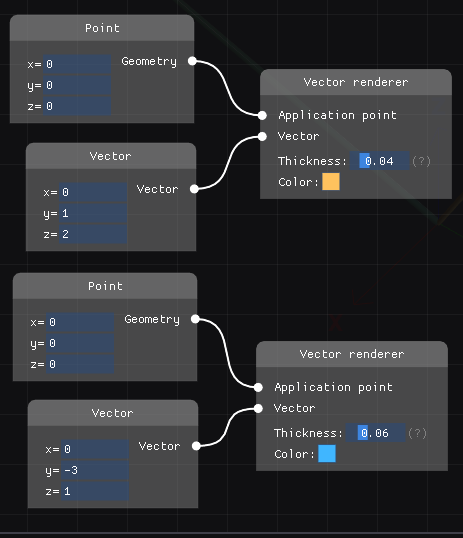
\includegraphics[width=0.50\textwidth]{\fig/lab2_es3_a.png}
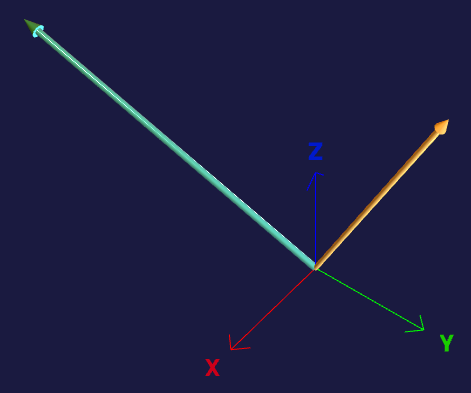
\includegraphics[width=0.35\textwidth]{\fig/lab2_es3_b.png}
\end{center}
\vspace{-0.25cm}
Notare come da alcune angolazioni i vettori potrebbero sembrare perpendicolari
anche se in realt\`a non lo sono.
\end{frame}

\begin{frame}
\frametitle{Esercizio 4}
        Dati i seguenti punti con relative coordinate: $A(1, 0, 1)$, $B(0, 2, 2)$, $C(1, 1, 3)$ e $D(2, -1, 2)$
\begin{itemize}
    \item Calcolare i vettori $\overrightarrow{AB}$ e $\overrightarrow{CD}$.
    \item Determinare se i due vettori siano paralleli.
    \item Rappresentare i due vettori nel \frnzplt.
\end{itemize}
\end{frame}

\begin{frame}
\frametitle{Esercizio 4 - i}
Determiniamo i due vettori:
\begin{displaymath}
\overrightarrow{AB} =  \begin{bmatrix}
                B_x - A_x \\
                B_y - A_y \\
                B_z - A_z 
                \end{bmatrix}
    = \begin{bmatrix}
                -1 \\
                2 \\
                1
                \end{bmatrix}
\qquad
\overrightarrow{CD} =  \begin{bmatrix}
                D_x - C_x \\
                D_y - C_y \\
                D_z - C_z 
                \end{bmatrix}
    = \begin{bmatrix}
                1 \\
                -2 \\
                -1
                \end{bmatrix}
\end{displaymath}

e proseguiamo impostando il sistema lineare come in precedenza:

$\overrightarrow{AB} \parallelsum \overrightarrow{CD} \quad \Leftrightarrow \quad \exists t \in \mathbb R, t\neq 0,\ \text{t.c. } \overrightarrow{AB} = t \overrightarrow{CD}$

\begin{equation*}
  \left\{
 \begin{array}{l}
  -1 = 1\ t \\
  2 = -2\ t \\
  1 = -1\ t
 \end{array}
 \right.
 \quad \rightarrow \quad
  \left\{
 \begin{array}{l}
  t = -1 \\
  t = -1 \\
  t = -1
 \end{array}
 \right.
\end{equation*}
\vspace{0.5cm}

Poich\'e $t=-1$ soddisfa tutte le equazioni del sistema, possiamo affermare che
$\overrightarrow{AB}$ e $\overrightarrow{CD}$ sono paralleli.
\end{frame}

\begin{frame}
\frametitle{Esercizio 4 - ii}
\vspace{-0.5cm}
\begin{center}
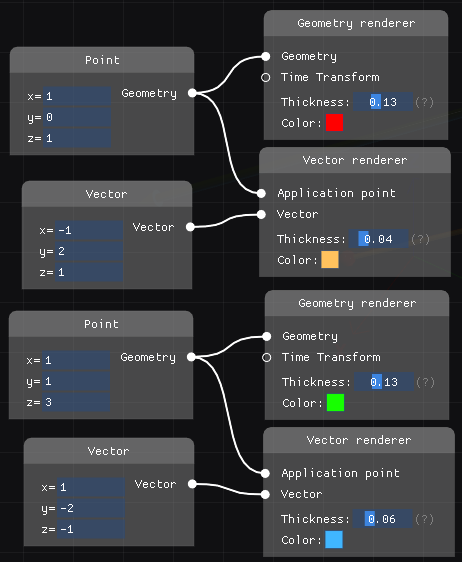
\includegraphics[width=0.50\textwidth]{\fig/lab2_es4_a.png}
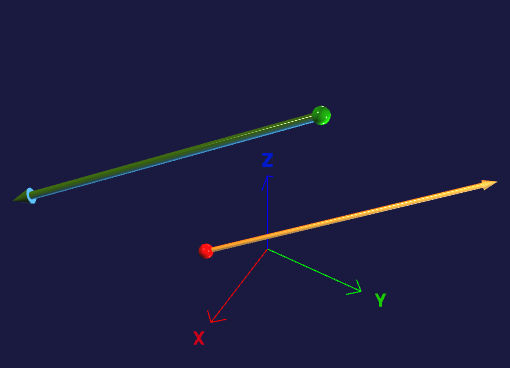
\includegraphics[width=0.45\textwidth]{\fig/lab2_es4_b.png}
\end{center}
\vspace{-0.25cm}
Per disegnare correttamente i vettori, \`e fondamentale spiccarli correttamente!\\ ($\overrightarrow{AB}$ parte da A, $\overrightarrow{CD}$ parte da C!)
\end{frame}

\begin{frame}
\frametitle{Esercizio 5}
    Dati i due vettori $\mathbf{u} = [1, 1, -2]^T$ e $\mathbf{v} = [0.5, -0.5, -0.5]^T$:
\begin{itemize}
    \item Calcolare il vettore $\mathbf{w} = \mathbf u \times \mathbf v$
    \item Rappresentare nel \frnzplt i tre vettori, con l'origine degli assi come punto di applicazione.
    \item Rappresentare nel \frnzplt il piano passante per l'origine e avente normale $\mathbf w$.
        Verificare che $\mathbf u$ e $\mathbf v$ giacciono sul piano.
    \item Cosa cambierebbe se anzich\'e $\mathbf w$ usassimo $\tilde{\mathbf{w}} = \mathbf v \times \mathbf u$?
\end{itemize}
\end{frame}

\begin{frame}
\frametitle{Esercizio 5 - i}
Ricordiamo la formula generica per il calcolo del prodotto vettore:
\begin{displaymath}
\mathbf a \times \mathbf b = 
\left[ \begin{array}{c} a_y b_z - b_y a_z \\ b_x a_z - a_x b_z \\ a_x b_y - b_x a_y \end{array} \right]
\end{displaymath}
Nel nostro caso:
\begin{displaymath}
\mathbf u \times \mathbf v = 
    \left[ \begin{array}{c} 
        1 \cdot (\shortminus 0.5) - (\shortminus 0.5) \cdot (\shortminus 2) \\
        0.5 \cdot (\shortminus 2) - 1 \cdot (\shortminus 0.5) \\
        1 \cdot (\shortminus 0.5) - (0.5) \cdot 1
    \end{array} \right]
=
    \left[ \begin{array}{c} 
        \shortminus 0.5 - 1 \\
        \shortminus 1 + 0.5 \\
        \shortminus 0.5 - 0.5
    \end{array} \right]
=
    \left[ \begin{array}{c} 
        \shortminus 1.5 \\
        \shortminus 0.5 \\
        \shortminus 1
    \end{array} \right]
\end{displaymath}

Abbiamo quindi trovato il risultato che cercavamo:

\begin{displaymath}
\mathbf w = 
    \left[ \begin{array}{c} 
        \shortminus 1.5 \\
        \shortminus 0.5 \\
        \shortminus 1
    \end{array} \right]
\end{displaymath}

\vspace{0.5cm}

\end{frame}

\begin{frame}
\frametitle{Esercizio 5 - ii}
\begin{center}
\begin{tikzpicture}
\node(img1){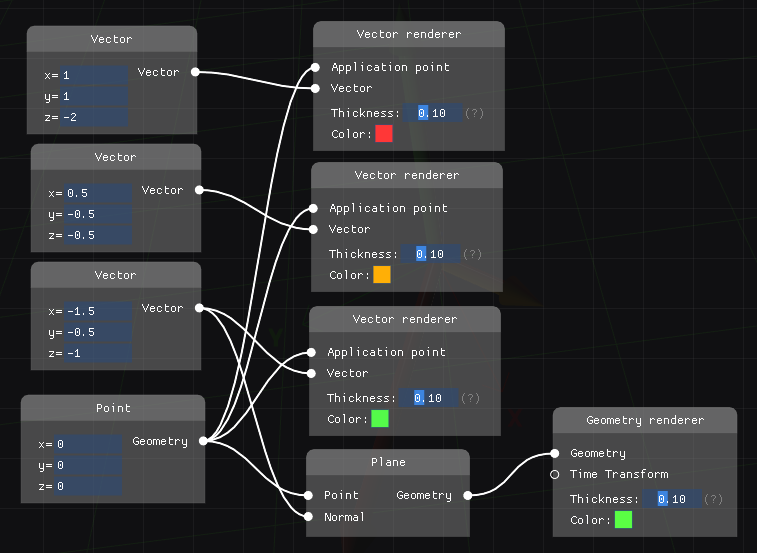
\includegraphics[width=0.8\textwidth]{\fig/lab2_es5_a.png}};
\node(img2) at (img1.east){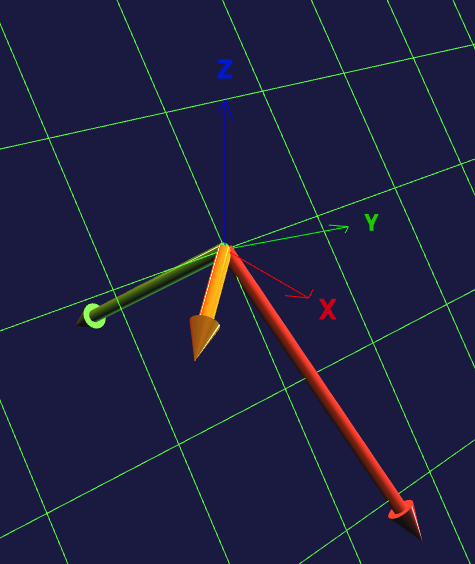
\includegraphics[width=0.25\textwidth]{\fig/lab2_es5_b.png}};
\end{tikzpicture}
\end{center}
\end{frame}

\begin{frame}
\frametitle{Esercizio 5 - iii}
Dalla teoria sappiamo che
\begin{displaymath}
\mathbf{b} \times \mathbf{a} = - (\mathbf{a} \times \mathbf{b})
\end{displaymath}
ovvero invertendo l'ordine del prodotto vettoriale otteniamo un vettore con i segni opposti rispetto al precedente.

\begin{displaymath}
\tilde{\mathbf w} = 
\shortminus \mathbf w = 
    \left[ \begin{array}{c} 
        1.5 \\
        0.5 \\
        1
    \end{array} \right]
\end{displaymath}

\vspace{0.5cm}

Dal punto di vista geometrico, significa che il vettore ha stesso modulo e direzione, ma verso opposto.

\end{frame}

\end{document}
